


\chapter{ Experimental Setup}

\section{Thomas Jefferson Lab}
\paragraph{}Thomas Jefferson Lab (Jlab) in Newport News, Virgina hosted the MARATHON experiment in the Fall of 2017 and Spring of 2018. Jlab uses support from the U.S. Department of Energy(DOE) and the state of Virgina to complete the lab's mission of delivering productive research by exploring the atomic nucleus and its fundamental constituents, including precise tests of their interactions. Along with applying an advanced particle accelerator, particle detectors and other technologies to develop new basic research capabilities and to address the challenges of a modern society.
	\subsection{CEBAF}\label{sec:cebaf}
	\paragraph{}The Continuous Electron Beam Accelerator Facility (CEBAF) was recently upgraded to a 12 GeV accelerator, upgrading it to be able to supply a 11 GeV beam of continuous electrons of up to 200 $\mu$A of current to three experimental halls (A,B,C) and 12 GeV to the recently constructed hall D. After being accelerated to 45 MeV by a polarized electron gun or a thermionic injector, the electrons are injected into the North linear accelerator (LINAC), shown in figure \ref{CEBAF}. The polarized gun can supply electrons with up to 80$\%$ polarization and the polarization direction can be controlled by a wien filter. To ensure the level of polarization, a 5 MeV Mott polarimeter may be used to measure the level of polarization\cite{HallA}.
	\paragraph{} The electrons are conveyed through two LINACs and two bending arcs per complete pass of the accelerator. Electrons traveling to Halls A, B, and C complete a maximum of four and a half revolutions around the accelerator. Electrons going to all D travel through the north LINAC for an extra boost. These particles receive approximately 2.2 GeV in energy for each cycle through the accelerator. The radio frequency (RF) cavities in each LINAC use an oscillating electromagnetic field to supply a force to accelerate the passing electrons. These Niobium RF cavities are cooled to 2 K in order to create conditions that allow the cavities to be superconducting \cite{HallA}.    
	
	\begin{figure}[h]
	\centering
	 \caption{Schematic Layout of CEBAF. }
	 \label{CEBAF}
	 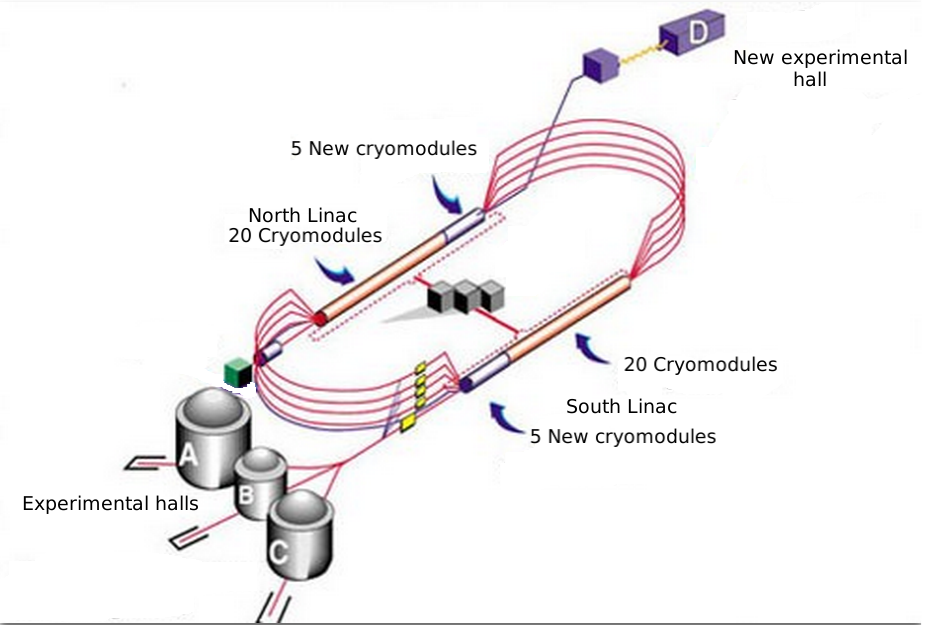
\includegraphics[width=10cm]{CEBAF.png} 
	 \end{figure} 
	 
	 \section{Hall A Beam Line}\label{sec:halla}
	 
	\begin{figure}[H]
		\centering
		\caption{A 3D drawing of Hall A. }
		\label{HallA}
		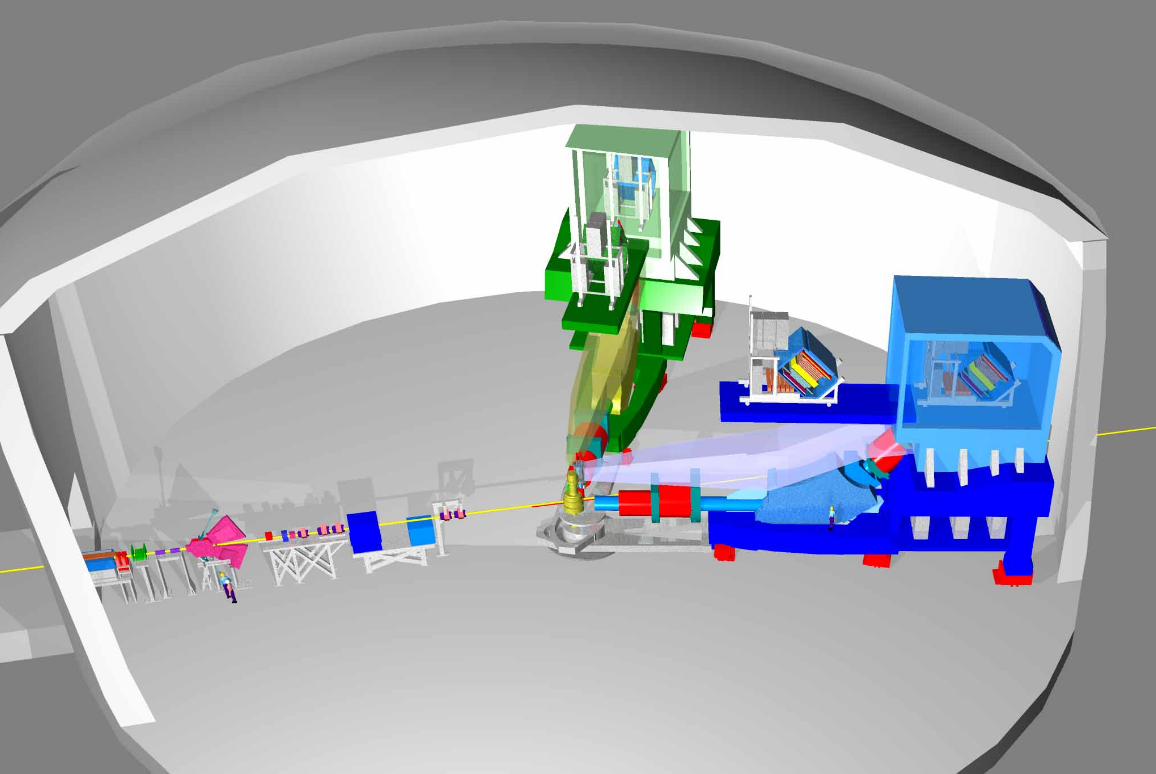
\includegraphics[width=14cm]{HallA_2.png} 
	\end{figure} 	 
	 
	 \paragraph{}The experimental Hall A and the scientific equipment used were designed for detailed investigations of the internal structure of nuclei. Two high resolution spectrometers in Hall A use the inclusive (e,e$\prime$) and exclusive (e,e$\prime$ p) reactions to gain a greater understanding of the structure of the nucleus. Completing detailed studies with high resolution and extreme accuracy requires knowing the beam position, size, energy, and current when the beam strikes the target. The instrumentation used in the precise measurement of these quantities in Hall A  are shown in figure \ref{BeamLine} \cite{HallA}. The information provided by these detectors originate through small changes in current and voltage sent through the electronics. These signals are transformed into useful information through calibrations.
 
	 \subsection{Beam Position Monitors}
	 \paragraph{} A pair of Beam Position Monitors(BPM)s are used to measure the relative beam position without affecting the beam. The two Hall A BPMs are located at 7.524 m and 1.286 m away from the target. Using the standard difference-over-sum technique, the relative beam position is determined with an accuracy of 100 $\mu$m with a beam current of at least 1 $\mu$A \cite{HallA}. The BPMs' positional data is recorded in two ways. Every second of beam time, the beam position average over 0.3 seconds is logged into the Experimental Physics and Industrial Control System (EPICS) database. The BPMs also transmit data event-by-event to the CEBAF online Data Acquisition system(CODA).
	 	 	 
 	 	\begin{figure}[H]
 	 		\centering
 	 		\caption{A schematic layout of the beam line in Hall. \cite{HallA} }
	 	 	\label{BeamLine}
	 	 	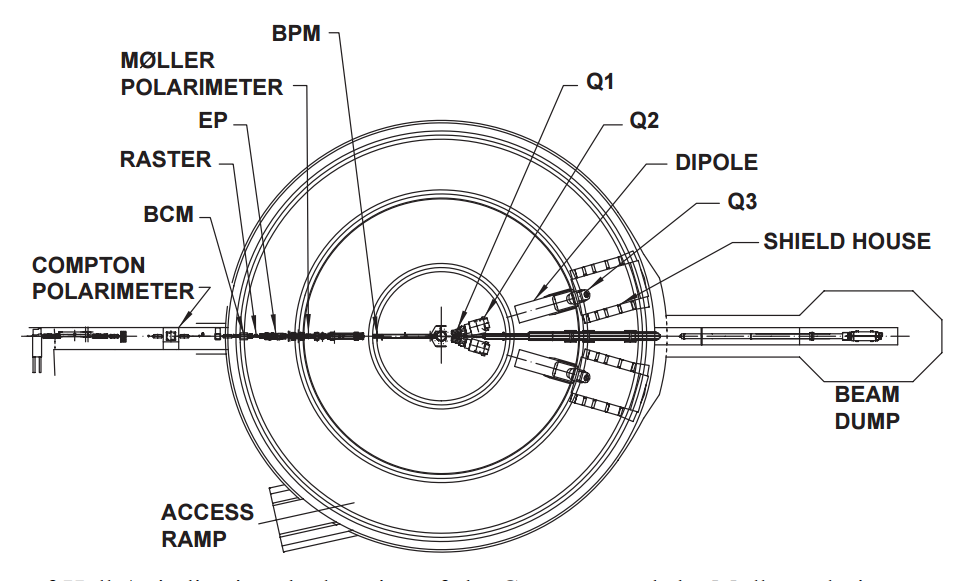
\includegraphics[width=14cm]{BeamLine.png} 
	 	 \end{figure} 	
	 	 	
	 \paragraph{} The main beam line components of the BPMs consist of four open-ended antennas. Figure \ref{BPMimg} shows a BPM chamber and figure \ref{BPM_4} shows the layout of the four antennas as you look down the beam line. In this chamber, the design of three of the four antennas can be seen. The antennas are titled $u_+$, $u_-$ and $v_+$, $v_-$. The antennas receive an induced signal as electrons pass to determine the beam position in the u and v directions. The BPMs send a DC offset to the DAQ. This DC offset is turned into a positional measurement via looking at both signals in one direction. The position in the frame of the u and v antennas are calculated by the taking the difference over the sum of the two wires in the u and v directions. The accuracy of the BPMs requires an absolute measurement of the electron beam's position to calibrate the BPMs\cite{BPM,BPM2}.
	 	 	\begin{figure}[H]
	 	 		\centering
	 	 		\caption{BPM design diagram, from JLab instrumentation	group. Beam direction is from left to right \cite{BPM2}. }
	 	 		\label{BPMimg}
	 	 		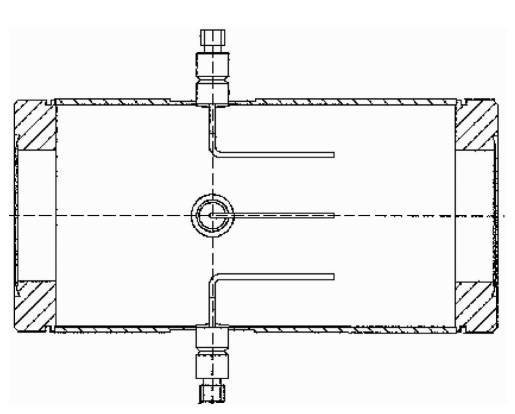
\includegraphics[width=10cm]{BPM.png} 
	 	 	\end{figure} 	
	 
	 %		\begin{figure}[H]
	 %			\centering
	 %			\caption{BPM design diagram, looking down the beam line\cite{BPM2}. }
	 %			\label{BPM_4}
	 %			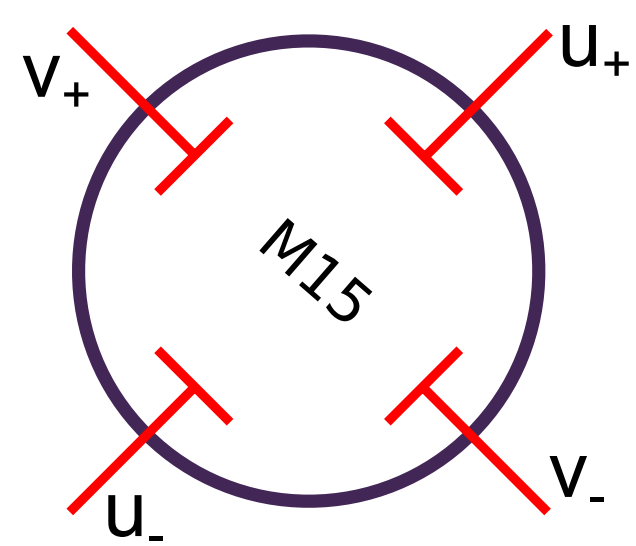
\includegraphics[width=10cm]{BPM_4.png} 
	 %		\end{figure} 
		\paragraph{} Two harps were used to provide the absolute measurement required for the calibrations. Each harp is located immediately after the BPM on the beam line. The harp forks are aligned perpendicular to the beam line to allow the harps to be moved in and out of the beam line. A wire that transverse between the fork tines at three different angles in respect to the harp is used to determine the horizontal and vertical position of the beam. The two sloped sections of the wire are angled at 45$^{\circ}$ relative to the harp frame. As the harp fork is moved into the beam, the wires receive a signal as the beam interacts with the wires. The two sloped wires are used together to determine the vertical position of the beam. The vertical wire is used to determine the horizontal position of the beam \cite{BPM,BPM2}. The harps are not used during production phases due their intrusive nature caused by the interaction of the beam with the harp wire.
		\begin{figure}[H]
			\centering
			\caption{A schematic layout of a harp fork \cite{BPM2} }
			\label{harp}
			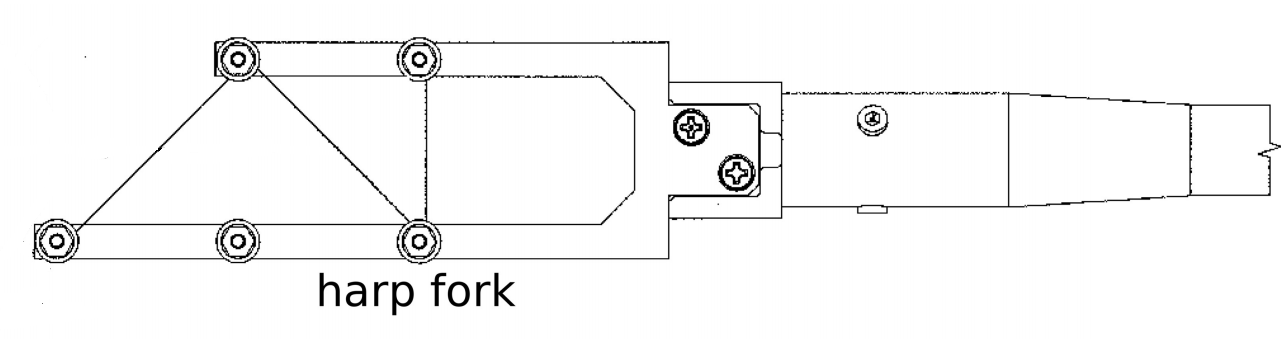
\includegraphics[width=14cm]{harp.png} 
		\end{figure}  	
		
		\paragraph{}The location of the wires on the harp frame and the position of the harp fork were used to calculate the absolute beam position. Figure \ref{bulls} shows an example of five positions used to calculate the BPM calibration coefficients. This method of using beam positions at the nominal center and surrounding the center is called a bull's eye scan. The harp scan results are substituted into equation \ref{BPM_eq} for the X and Y positions. Using all five points and an $R^2$ regression technique, the coefficients can be determined with great accuracy. These highly accurate BPMs were crucial in reducing systematic error in the final results obtained from this experiment. 
		\begin{equation}
		\label{BPM_eq}
		\begin{pmatrix}
		X_{position}\\
		Y_{position}
		\end{pmatrix}
		=
		\begin{pmatrix}
		C(0,0) & C(0,1)\\
		C(0,0) & C(0,1)\\
		\end{pmatrix}
		*
		\begin{pmatrix}
		X_{BPM}\\
		Y_{BPM}
		\end{pmatrix}
		+
		\begin{pmatrix}
		X_{offset}\\
		Y_{offset}
		\end{pmatrix}			 
		\end{equation}
		
		\begin{figure}[H]
			\centering
			\caption{The X and Y position for a Bulls eye scan for BPM calibration. }
			\label{bulls}
			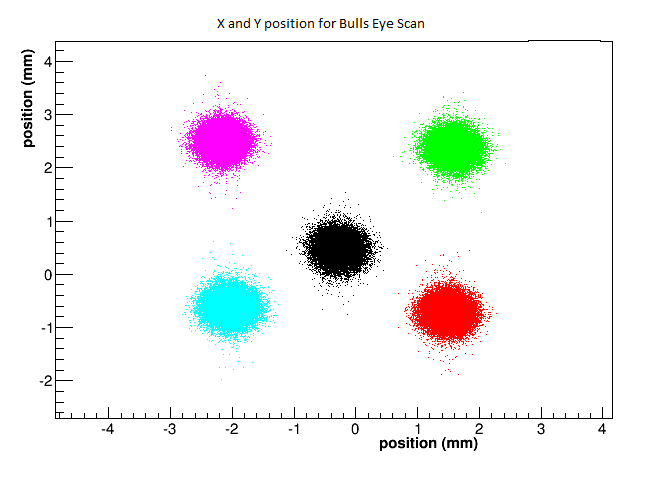
\includegraphics[width=10cm]{bulls.png} 
		\end{figure} 	

	 \subsection{Raster}
	 \paragraph{} Damage to a target system from intense beam can cause extreme fluctuations in the target's temperature and density. A raster was used to counteract the damage caused by a focused beam. The raster used two magnetic fields produced by two dipoles to spread the electron beam out. This produces a large rectangle interaction area on the front face of the target container. A triangle wave of 25 kHz was used to control the coils of the dipole magnets. The raster systems are located $\approx$17 meters before the target chamber (upstream of the target\cite{BPM2}). The rasters position can be seen in figure \ref{HallA}. Safety constraints administrated by the target group at JLAB limited the minimum size of the raster spot for the MARATHON experiment to two millimeters by two millimeters. This limit was installed has a safety concern for the tritium target. 
	 \paragraph{} The Hall A raster system consists of four dipoles. Two dipoles produce magnetic fields in the horizontal direction of the lab frame and two in the vertical. The upstream raster and downstream rasters include one vertical and one horizontal dipole. The relative change in position of the incoming electrons are controlled by the current supplied to the dipoles. This current that drives the dipoles is recored by an ADC. In order to obtain the change in beam position due to the rasters, a calibration between the raster current and measured beam position were obtained.  
	  \begin{figure}[h]
	 	\centering
	  	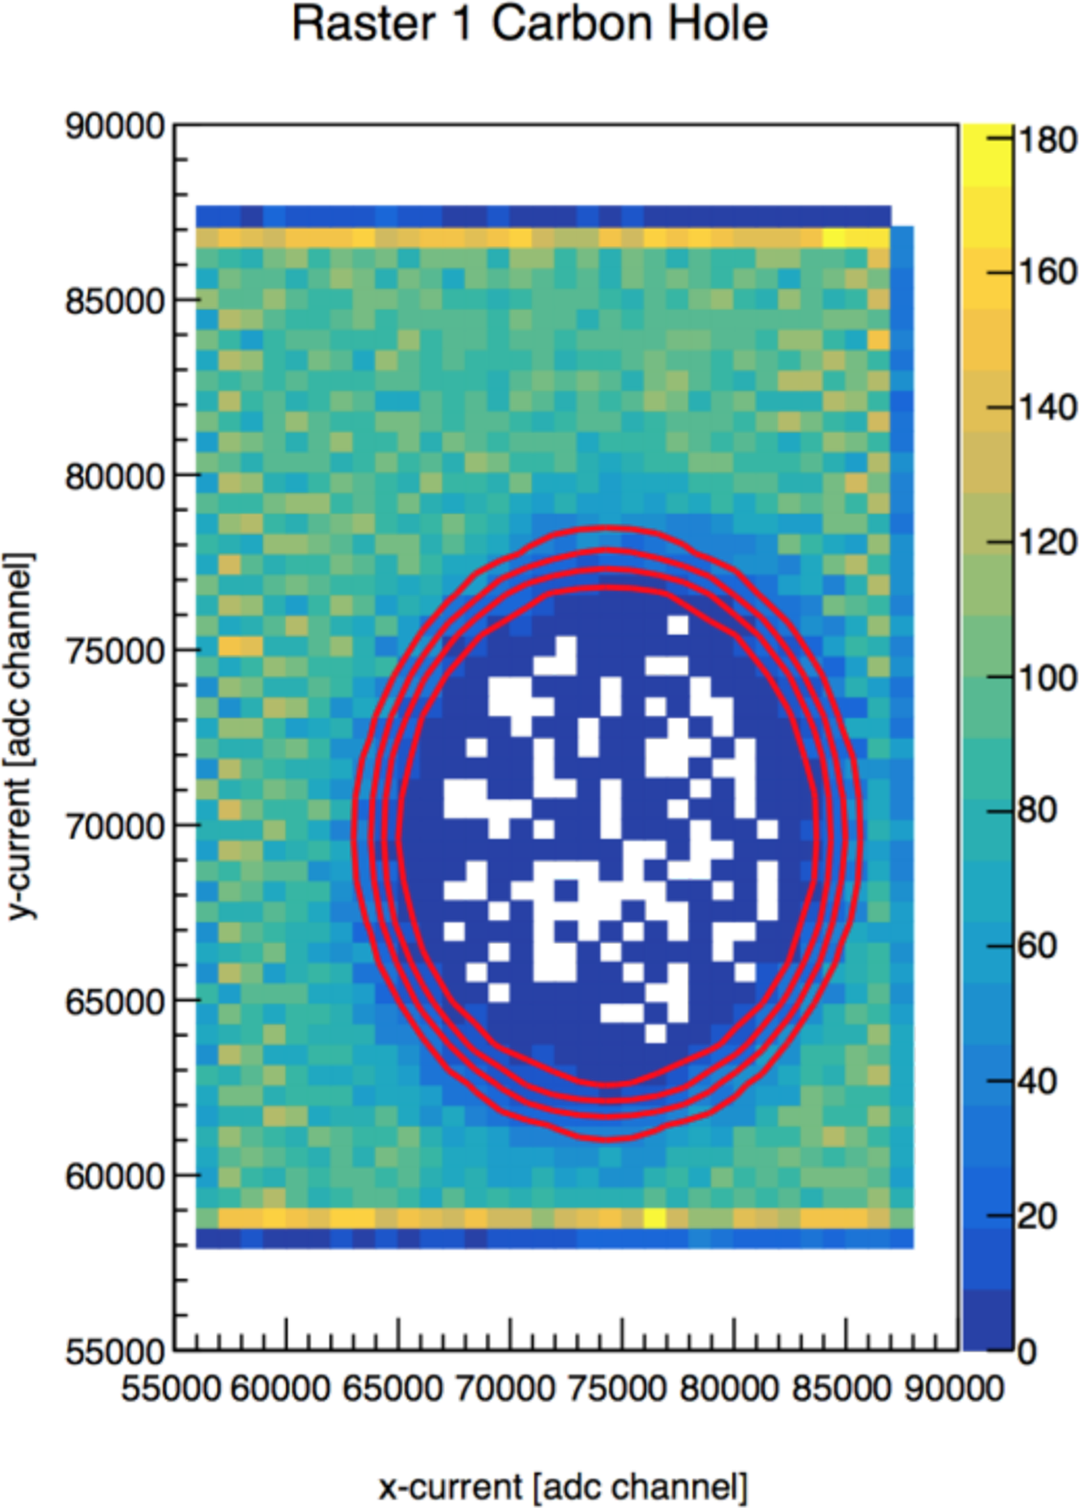
\includegraphics[width=7.5cm]{raster.pdf} 
	 	\caption{The X and Y current of the raster with a carbon hole. The size of the carbon hole is fit with a radial sigmoid\cite{Trast}.}
	 	\label{fig:raster}
	 \end{figure} 
	 \paragraph{}
	 The raster calibration is done by creating a line that maps the raster current measured by ADC bins to a position. This calibration process is done to extract positions at the locations of both BPMs and the target center along the beam line. The calibration of the linear mapping of raster current to beam position took two process. The first process was to determine the size of the rastered beam spread. In order to accurately determine the width and height of the beam spread due to the raster, a carbon foil with a hole of a diameter of 2mm was used. A radial sigmoid was used to fit the hole. The fit of the carbon hole gives the width of the raster, the slope of the linear mapping term. In figure \ref{fig:raster}, the raster current in x and y directions are fitted using this radial sigmoid. Once the slope of the linear calibration is determined, the offsets can be found. This is discovered by using the calibrated BPM mean positions for a phase of rastered beam. The mean positions for both BPMA and BPMB are used to produce a track from the BPMs to the target. This projection provides a mean location of the beam at the target.  Using equation \ref{eq:raster}, the offsets also know as the intercepts can be solved for using the slope ($m_x,m_y$), the raster mean current value ($R_x,R_y$), and the mean BPM position($x,y$).  \cite{Trast} 
	 \begin{equation}
	 	\begin{pmatrix}
	 	x\\
	 	y
	 	\end{pmatrix}
	 	=
	 	\begin{pmatrix}
	 	R_x\\
	 	R_y
	 	\end{pmatrix}
	 	*
	 	\begin{pmatrix}
		m_x && 0 \\
		0  && m_y
	 	\end{pmatrix}
	 	+
	 	\begin{pmatrix}
	 	O_x\\
	 	O_y
	 	\end{pmatrix}
	 	\label{eq:raster}
	 \end{equation}

 
	 \subsection{Beam Energy}
	 \paragraph{}The electron beam energy is located in many of the equations used in an electron scattering experiment. This can cause a noticeable increase in systematic error if the beam energy measurement is not made precisely. At JLAB for the MARATHON experiment, the beam energy was measured in two ways. In Hall A, the beam energy was measured by using the (e,e$\prime$p) method. On the beam line, 17 meters upstream from the target an ep scattering chamber is located. The beam was directed into the target containing a rotating 10-30 $\mu$m thick tape of C$H_2$. The scattering angle of the electron and the recoil angle of the proton are used to determine the beam energy using equation \ref{EP}. Where $M_p$ is the mass of the proton and $\theta_p, \theta_e$ are the scattered angle of the proton, electron respectively. 
	\begin{equation}
	\label{EP}
	E = Mp \frac{cos\theta_e + \frac{sin\theta_e}{tan\theta_p}-1}{1 - cos\theta_e} 
	\end{equation}
	The beam energy was also measured using the ark measurement method \cite{Flay}. This method uses changes is beam position and precise measurements of the magnetic fields around the beam line to determine the energy of the electron beam. The angle at which the electrons are bent through is related to the momentum of the electrons,
	\begin{equation}
	\label{arc}
	p = k \frac{\int \vec{B} \cdot d\vec{l}}{\theta}.
	\end{equation}	
	In equation \ref{arc}, p is the momentum of the electrons, $\theta$ is the bend angle, and $\vec{B}$ is the magnetic field the electron experiences. Then using the momentum of the electron, the energy of the beam can be extracted. The error on the beam energy measurement is $\delta$ E/E $\approx$ 2 $* 10^{-4} $ \cite{EPMet, Flay}.  The MARATHON experiment used both methods to accurately determine the electron beam energy.
	
		  	\begin{figure}[H]
		  	 	 		\centering
		  	 	 		\caption{Hall A Current Monitor components \cite{BCM1}. 
		  	 	 		\label{BCMpng}}
		  	 	 		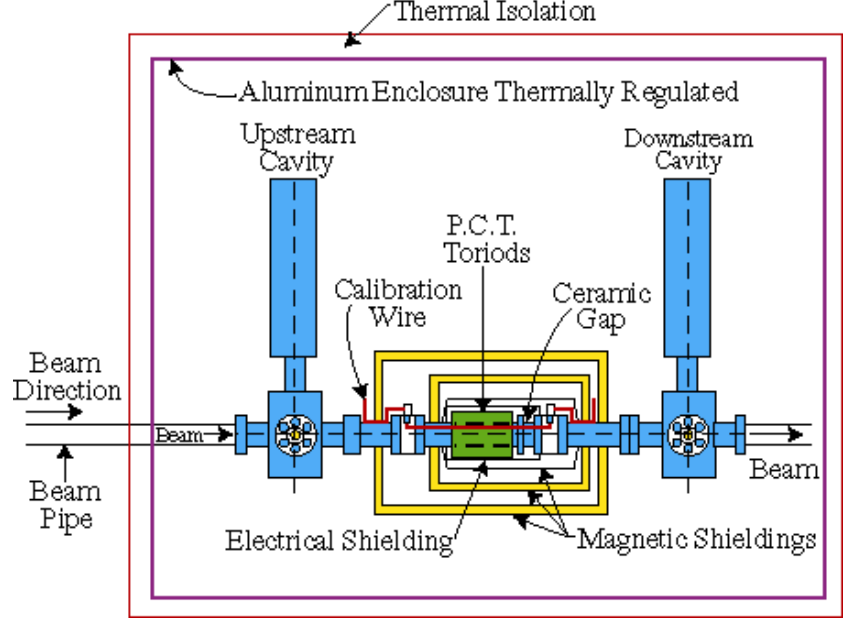
\includegraphics[width=10cm]{BCM1.png} 
		  	\end{figure}
	\subsection{Beam Current Monitors}
	\paragraph{} The main process of measuring the scattering yield for a calculation of a cross section looks at finding the ratio of the number of electrons scattered to the number of electrons sent. In order to accurately determine the number of electrons sent to scatter with our target system, Hall A use a set non-invasive beam current monitors(BCMs). The Hall A BCMs have an absolute accuracy of 0.2 percent as long as the current is between 1 and 180 $\mu$A. The BCMs used in Hall A consist of three main components: a Parametric Current Transformer (PCT) and two pill box cavities. Figure \ref{BCMpng} shows the components in the Hall A BCM.  The BCM produces an RF signal that is proportional to the beam current. A 10 kHz down converter, RMS-to-DC converter, voltage-to-Frequency converter, and a scaler are used to inject the current signal into the Hall A DAQ. Proportionality constants are determined in the calibration process to correctly integrate the charge for a given amount of beam current\cite{BCM1}.
	\begin{figure}[h]
		\centering
		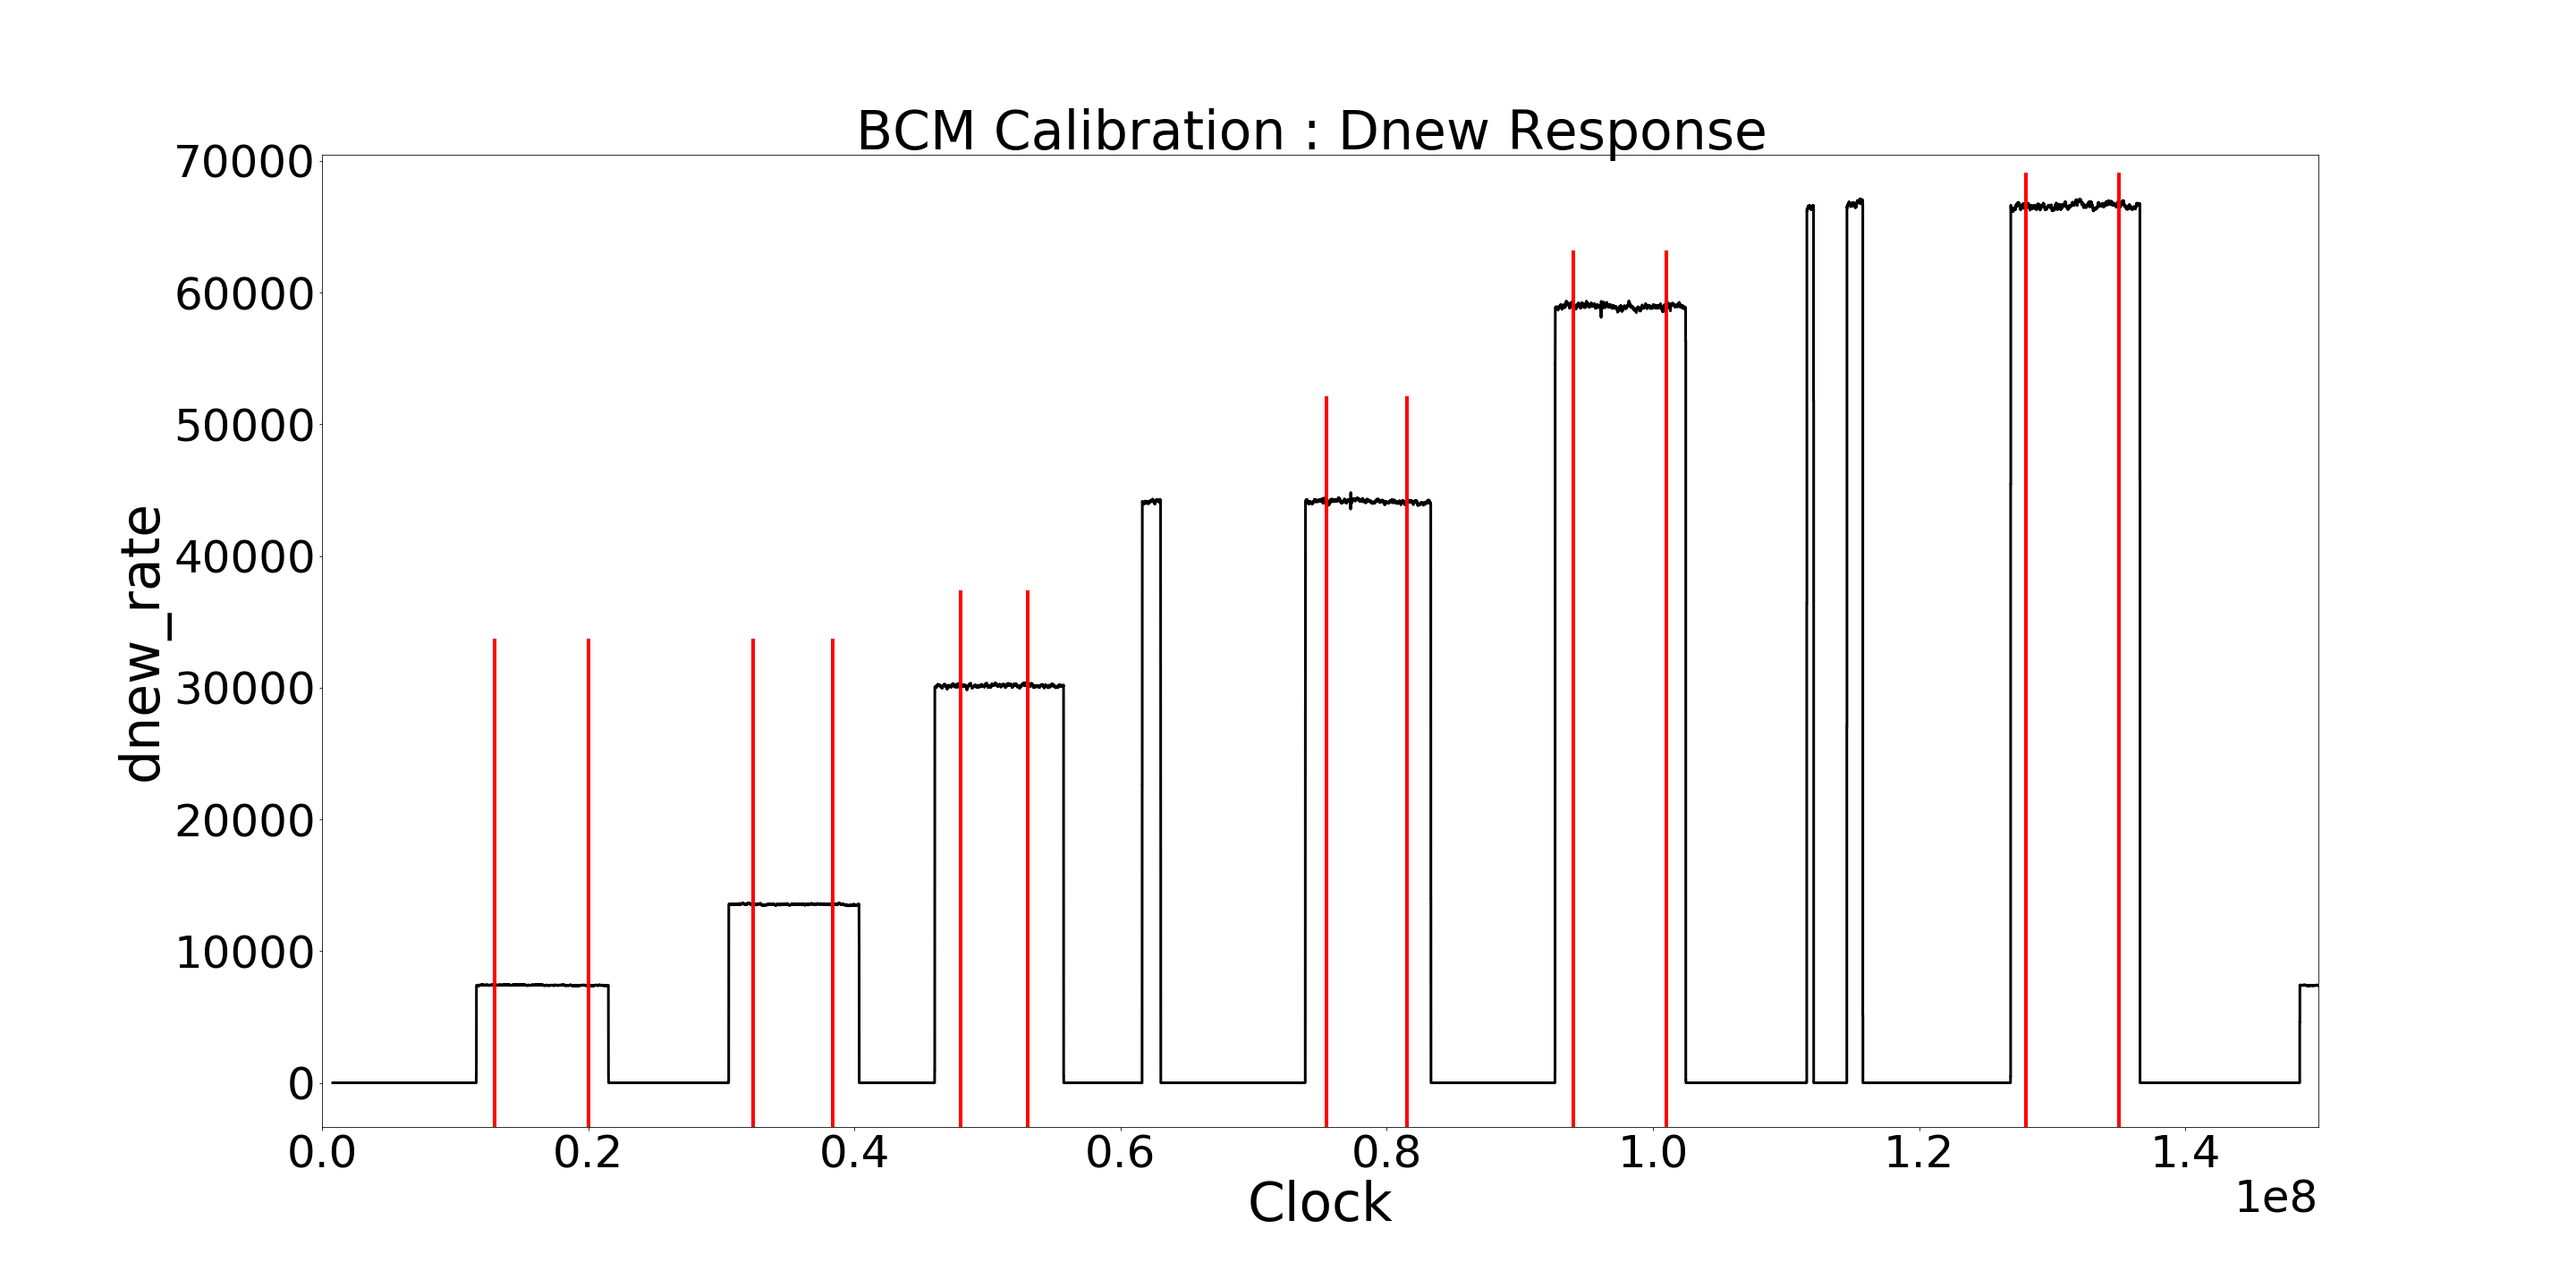
\includegraphics[width=17cm]{dnew_freq.png}
		\caption{BCM calibration \cite{MikeTh}.
		\label{dnewfreq}}
	\end{figure}
	The process of calibrating the BCM converts the frequency received from the BCMs to an amount of current in $\mu$A. In order to calibrate the BCMs in Hall A, a separate intrusive calibration of an unser must be done. The unser is calibrated by inserting a known current through a wire inside the beam pipe. The calibration of the unser is known to drift over time, which makes the unser unfeasible to use as the main source of charge calculation. Once the unser is calibrated, the BCM calibration procedure can be completed. The BCM calibration requires the delivery of the electron beam with unique procedure. This process consist of oscillating the beam on and off status while increasing the current. This process can be seen in figure \ref{dnewfreq}. This stepping up procedure provides an adequate number of data points to complete a linear fit of the BCM frequency verses the calibrated unser current. The linear fit parameters supply a multiplicative gain and an additive offset for the calibration of the BCMs. Figure \ref{bcmcal} shows a linear fit that provides gain and offset calibration constants for the BCM used in the calculation of charge. 
	\begin{figure}[h]
		\centering
		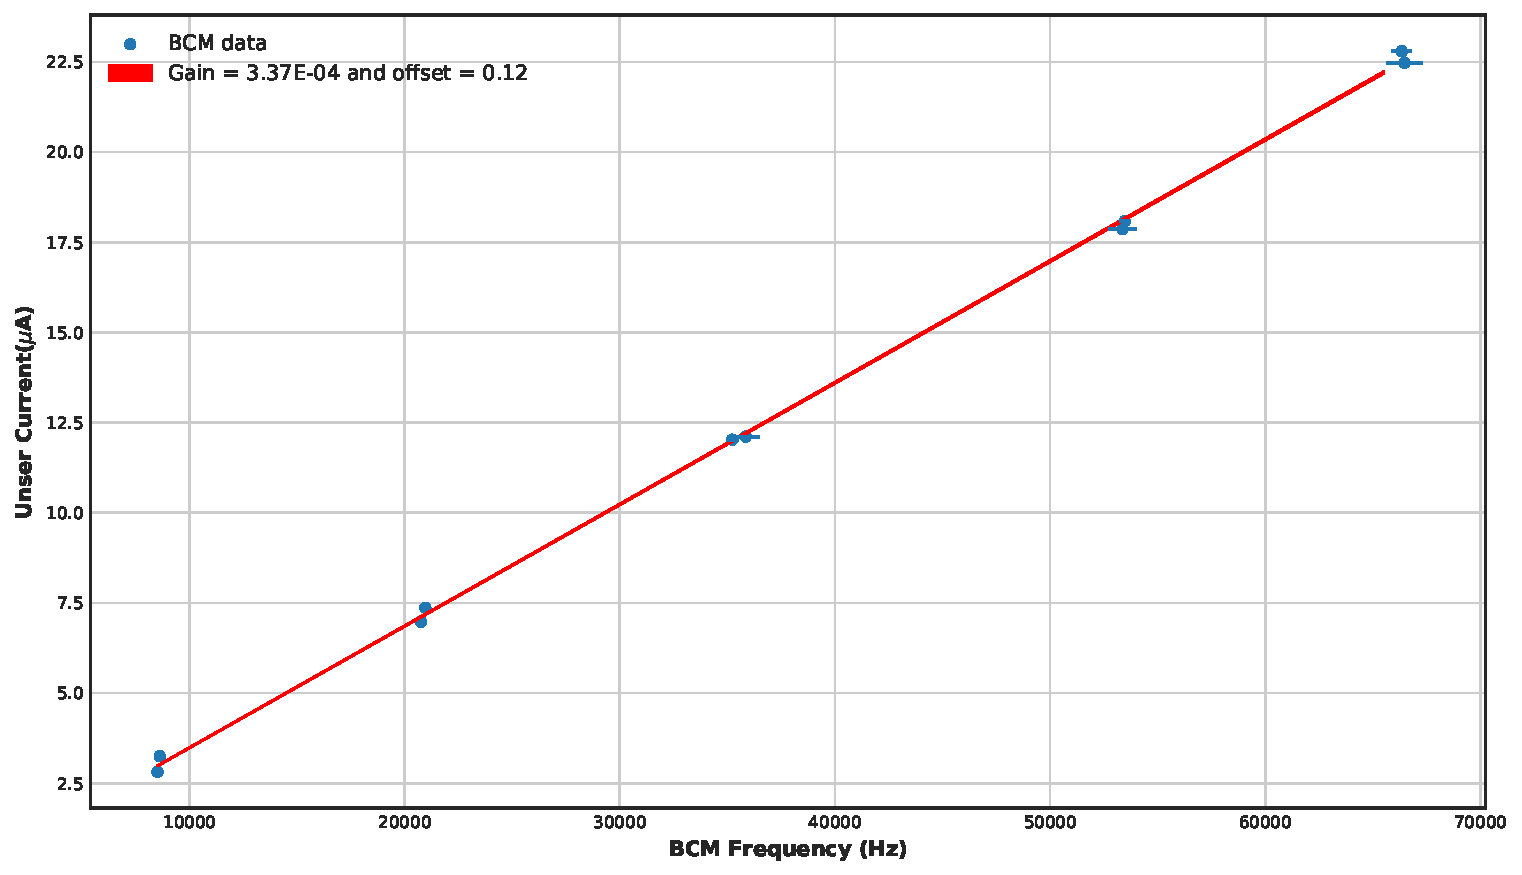
\includegraphics[width=12cm]{BCMcal.pdf}
		\caption{BCM frequency for BCM calibration \cite{MikeTh}.
			\label{bcmcal}}
	\end{figure}	
	  
\section{Target}\label{sec:target}
\paragraph{} The Hall A Tritium Target(HATT) system was used for the Tritium run group of experiments. The HATT target chamber was repurposed from a previously used cryo-target chamber in order to reduce the financial cost of designing a new target chamber. The refurbishing of the cryo-target chamber consisted of adding in new safety features to prevent and mitigate a tritium leak.  A 4 inch long collimator with an inner diameter of 0.4 inch was added inside of the target chamber but upstream of the target ladder to prevent the beam from striking the thin side wall of the aluminum cell. In case of a tritium leak in the target chamber, an exhaust system was installed to control the amount of tritium exposed to the Hall.\cite{HATT_eng}  Figure \ref{HATT} shows the HATT system with the target ladder in the home position and the scattering windows removed. 
\begin{figure}
	\centering
	\caption{Target Images}
	\hspace*{-20pt}
	\subfloat[A image of the HATT. \cite{DHimages}]{{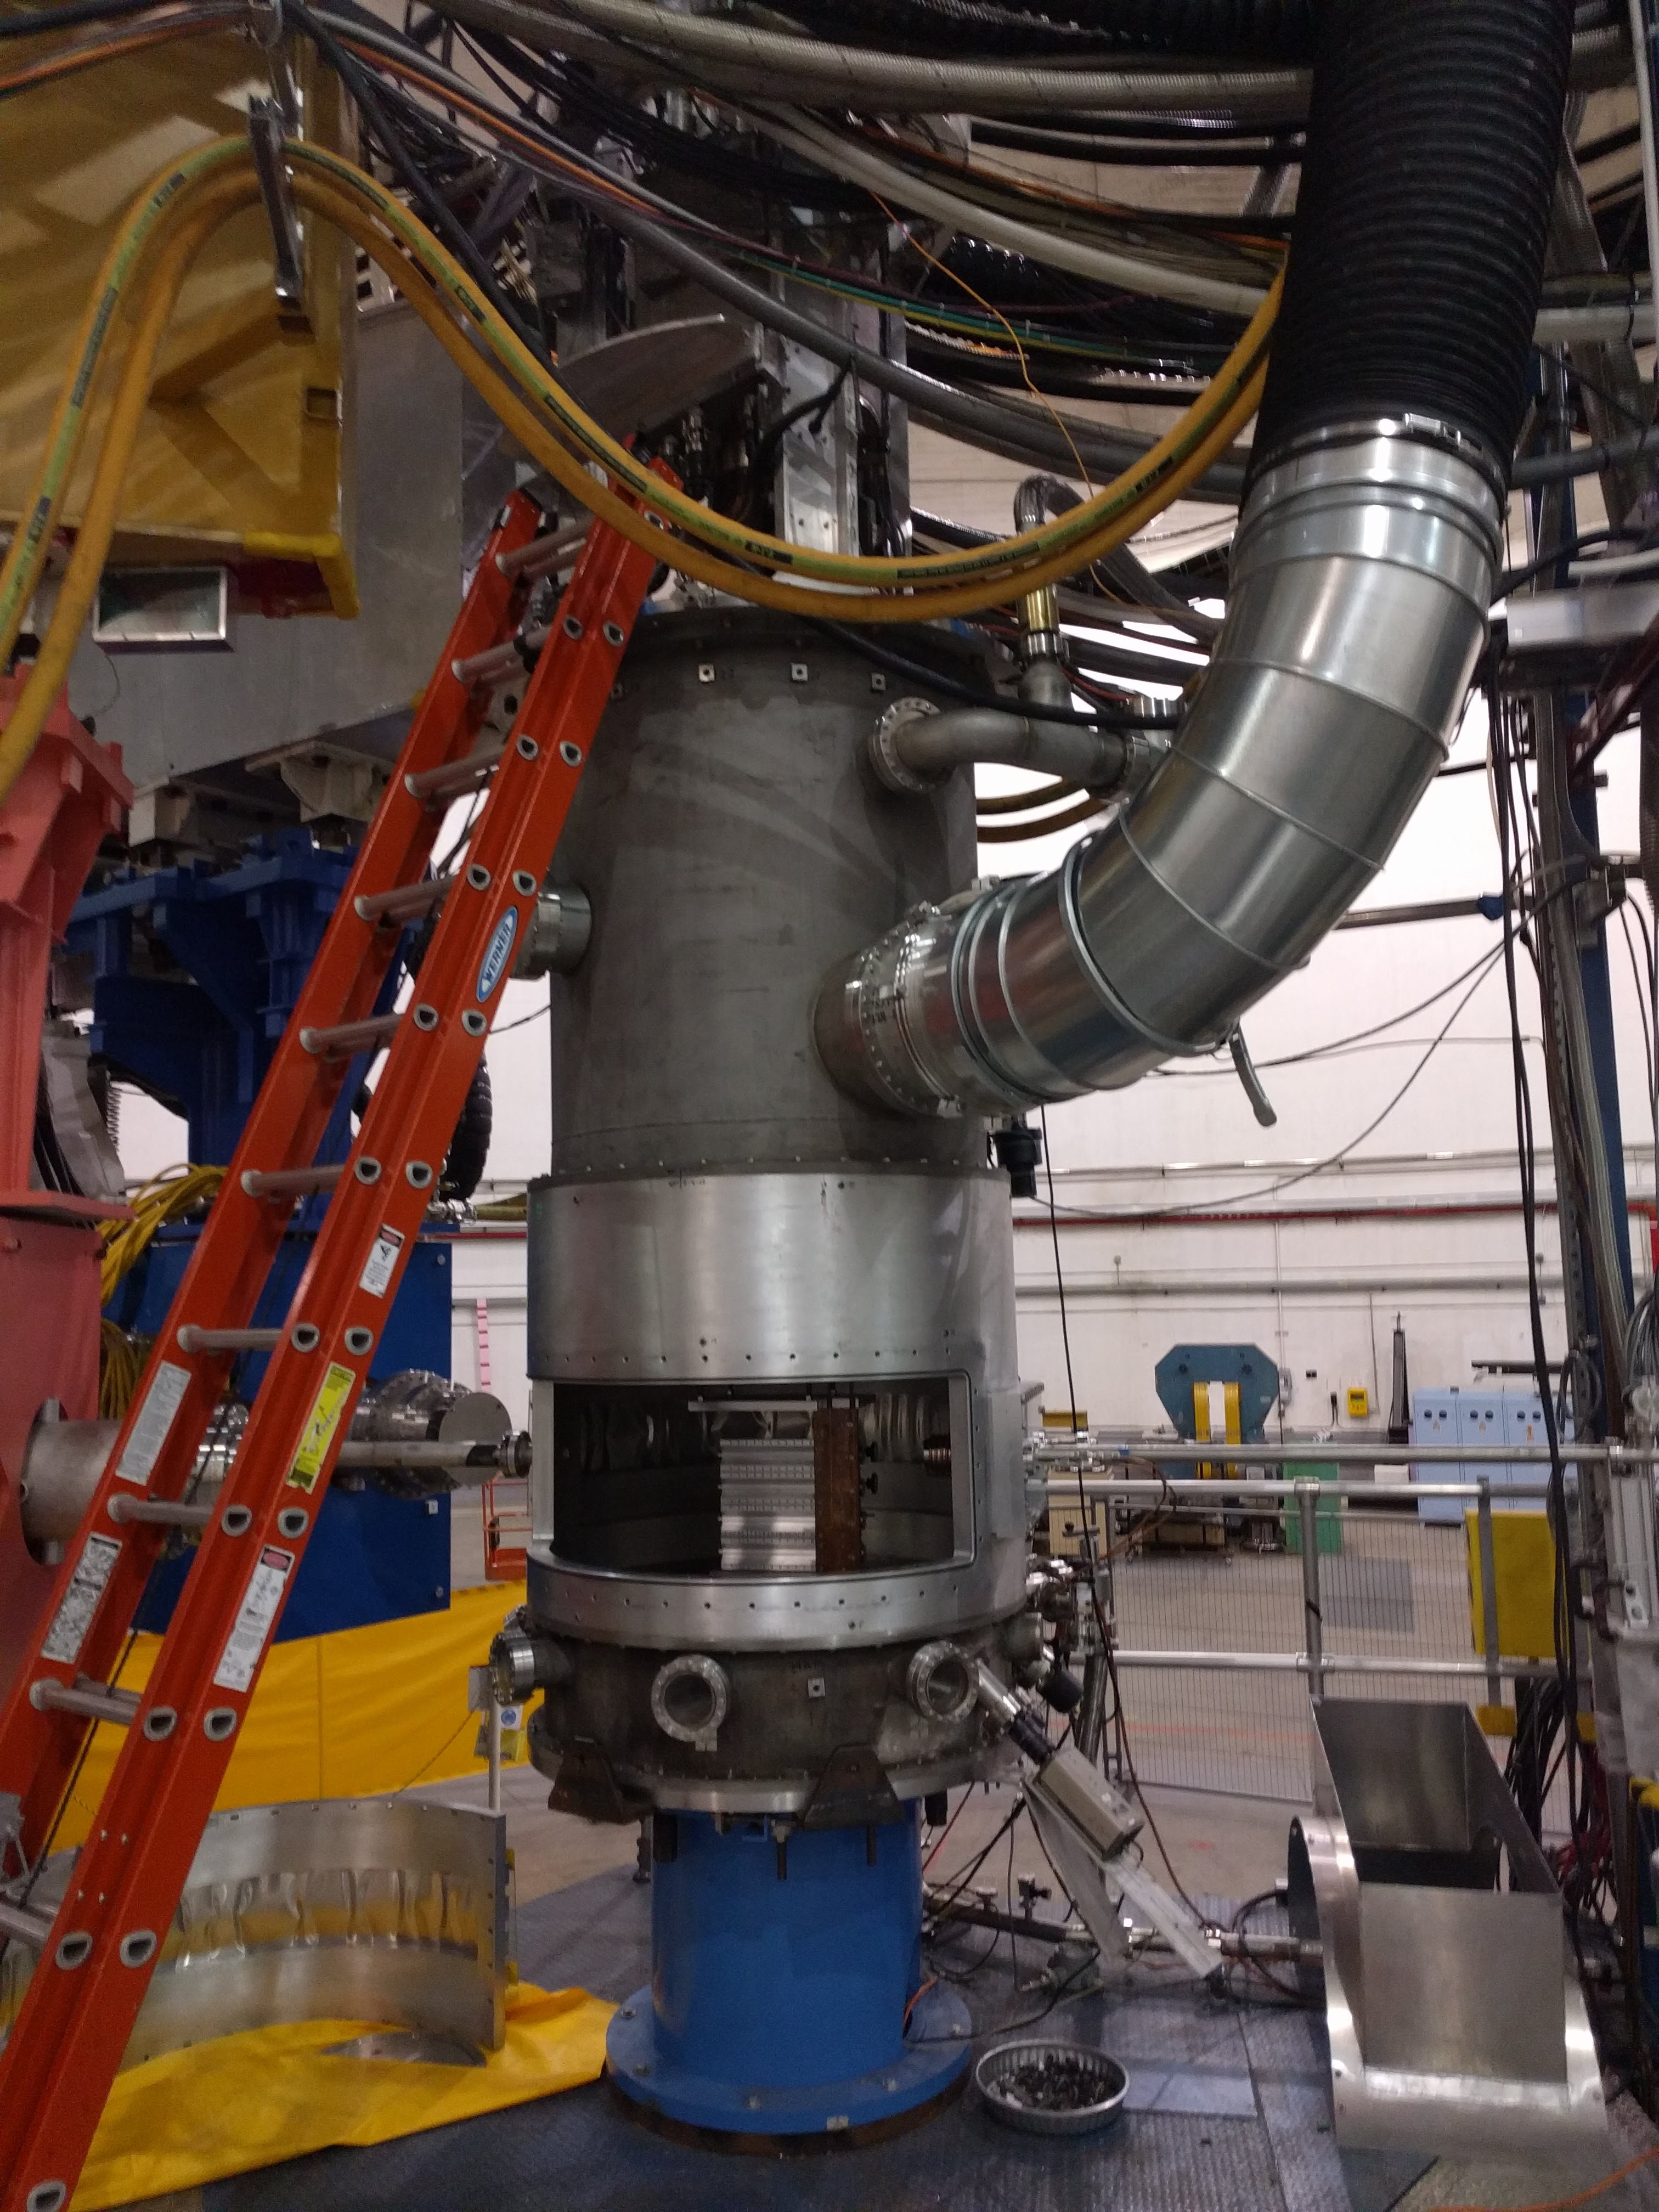
\includegraphics[width=6cm]{HATT.jpg} }}
	\quad
	\subfloat[Image of the Hall A Tritium Target Ladder. \cite{DHimages}]{{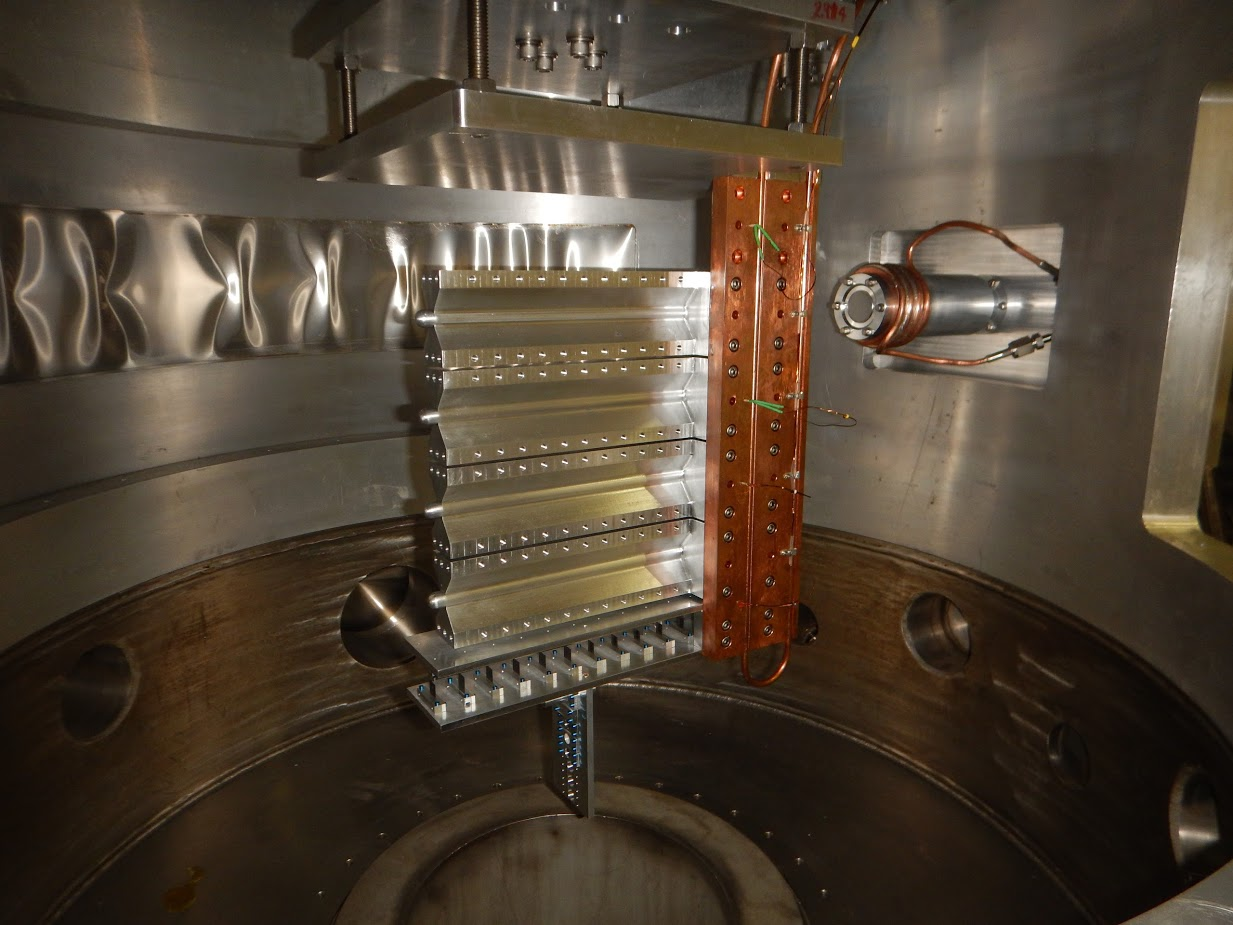
\includegraphics[width=10cm]{HATT_Ladder.JPG} }}
	\label{HATT}


\end{figure}
A picture of the HATT ladder installed in the HATT system is shown if figure \ref{HATT}. The ladder contains both gaseous cells and solid targets. The MARATHON experiment had five gas cells. The top four of the gas cells were filled with tritium, deuterium, hydrogen, and $^3$helium, from top to bottom respectively. Due to safety restricts the tritium cell was not installed until the HATT system could be closed. The bottom most cell was left empty, to complete end cap subtractions. The lower half of the target ladder contains the solid targets used during the MARATHON experiment. Listed from top to bottom, the solid targets used were a pair of thick aluminum foils, carbon multifoil, single carbon foil, and a carbon foil with a 2mm diameter hole. The thick Al foils were used to aid the target window background subtraction. The multifoil target also know has the optics target was used to calibrate the z-axis  reconstruction of the optics matrix. The single carbon foil and carbon hole were used to calibrate the BPMs and rasters and to determine the off set of the central line of the detector. 

\begin{figure}[h]
	\centering
	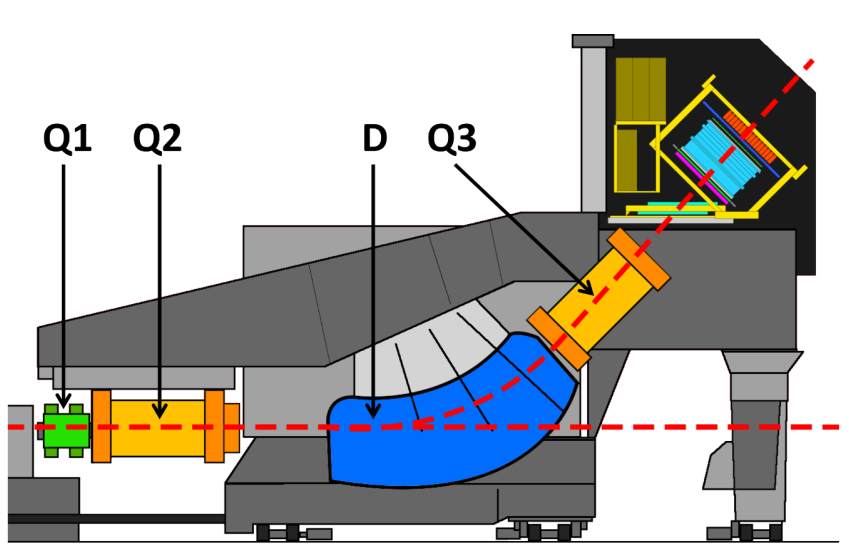
\includegraphics[width=10cm]{HRS_full.png}
	\caption{A side view of a HRS \cite{HallA}.
		\label{hrsfull}}
\end{figure}

\section{High Resolution Spectrometers}\label{sec:HRS}
Electrons that successfully scatter from the target may end up in either of the two HRSs(High Resolution Spectrometers). The HRSs were designed to detect charged particles with a high degree of precision. 
In order to achieve a high level of resolution in momentum and angle, the HRSs were designed with a magnet configuration of QQ$D_n$Q (quadrupole, quadrupole, dipole, and quadrupole). The vertical bending dipole provides the field required to transport the scattered particles through the 45$^\circ$ bending angle to the detector hut. A drawing of an HRS can be seen in figure \ref{hrsfull}. The first quadrupole(Q1) focuses the incoming electrons in the vertical plane. The following two quadrupoles (Q2 and Q3 provide transverse focusing. This optical design allows the use of extended gas targets with no substantial loss in solid angle\cite{HallA}.  The spectrometers were designed to perform various functions which include: triggering the data acquisition system (DAQ) when certain requirements are met, gathering the position and direction of individual particles to reconstruct a track, provide precise timing information for time of flight calculations, and identify many different particle types that pass through the detector system. In order for both the Left HRS (LHRS) and Right HRS (RHRS) to  complete the required task, they contain a myriad of detectors. The HRSs use drift chambers, scintillators, cerenkov detectors, and shower calorimeters. Both the Left and Right HRSs contain two planes of scintillators to function has the main trigger for the detector package. The vertical drift chambers (VDC) that lay at the front of the detector in conjunction with the Shower that lies in the back of the detector provide information for reconstructing the particle tracks and precise timing. Particles are identified by the cerenkov, shower calorimeters, and pion rejectors that are contained in the left or right HRS. The layout of the individual detectors that make up the left and right detector package are shown in figure \ref{hrsss}  \cite{HallA}.
\begin{figure}[t]
	\centering
	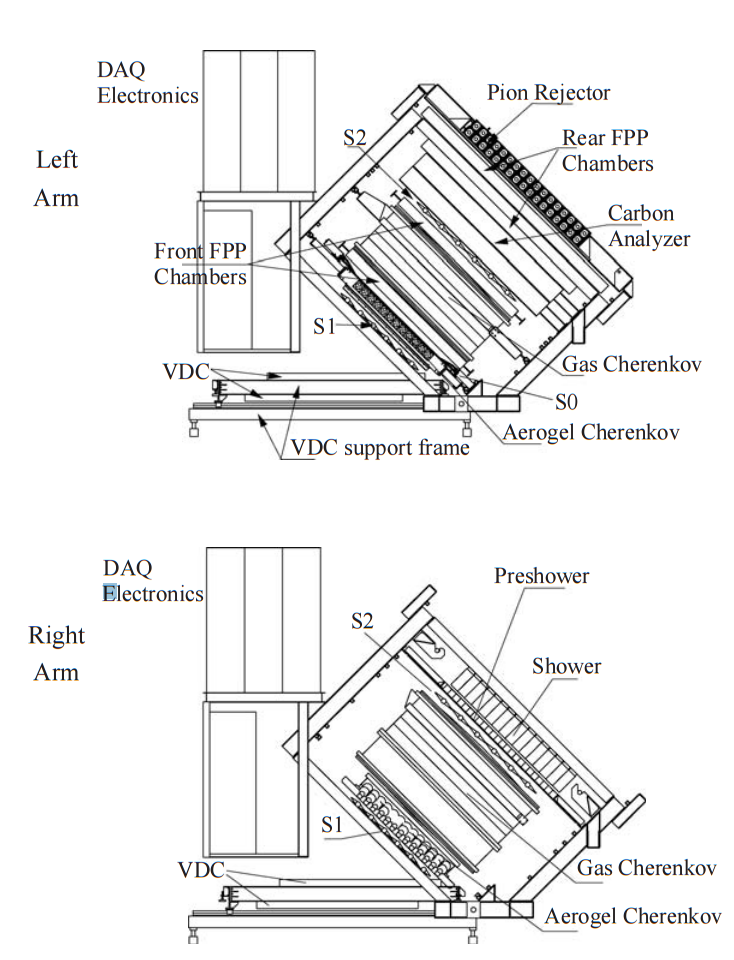
\includegraphics[width=10cm]{HRSs.png}
	\caption{A view of both the left(top) and right(bottom) detector stacks inside the left and right HRS \cite{HallA}.
	\label{hrsss}}
\end{figure}

	\subsection{Vertical Drift Chambers}\label{sec:vdc}
	\paragraph{}Each of the spectrometers housed in Hall A contains two vertical drift chambers(VDC). Each VDC incorporates two planes of crossing sense wires. Shown in figure \ref{VDC_profile}, the two planes of the VDC lie a distance of 0.335m apart \cite{drift}. The lower plane of the VDC is positioned at the approximate focal plane of the HRS and lies in the horizontal plane of the Hall A coordinate system. The sense wires located in the VDCs cross orthogonally. They are offset by $45^\circ$ in respect to the dispersive and non-dispersive directions. Each plane of the VDC uses 368 sense wires, with 4.24 mm between each wire. The signals from these wires are transmitted to the electronics via a set of printed circuit boards that contain a 16-channel connector and twisted pair ribbon cables. These ribbon cables transmit the VDC signal to a set of common stop TDC with 0.5 ns resolution \cite{drift}. The VDC sense wires are held at ground potential between two planes of high-voltage. Particles that enter the gas filled VDC, collide with molecules of an argon($62\%$) and ethane ($38\%$) mixture \cite{HallA}. This collision causes the ionization of the gaseous mixture producing drift electrons.
	\begin{figure}
		\centering
		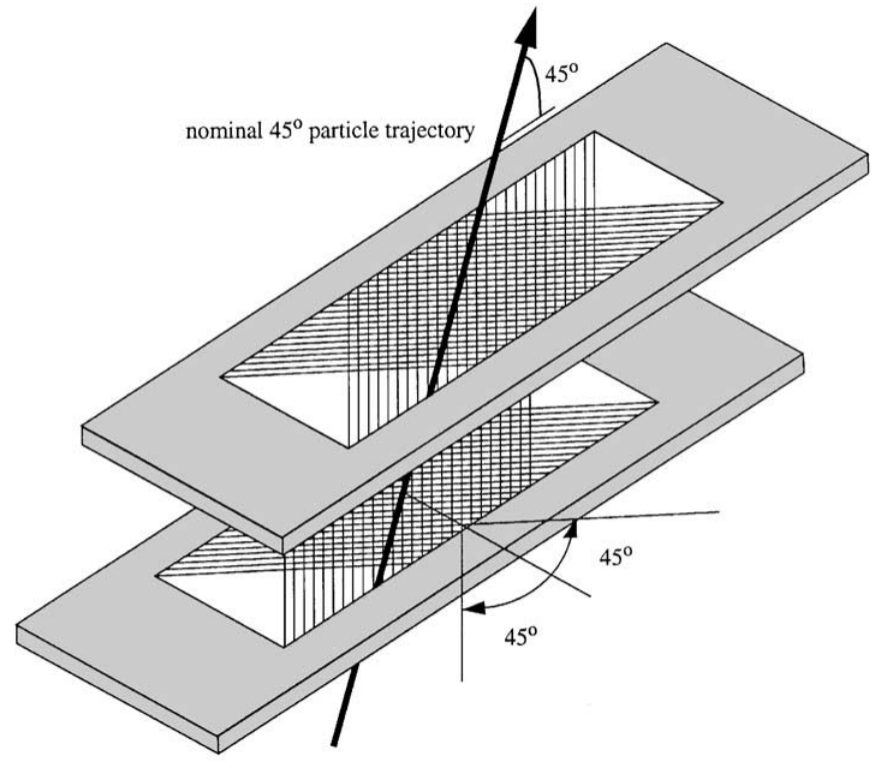
\includegraphics[width=10cm]{VDC_profile_view.png}
		\caption{A sketch of the two VDC planes in the HRSs with a particle traveling through the detector at 45$^\circ$.\cite{drift}.
			\label{VDC_profile}}
	\end{figure}
	\paragraph{} Particles that transverse the VDCs will travel through regions close to several sense wires. As the indecent particle ionizes gas in each of these regions, the VDC sense wires pick up the corresponding signal from the drift electrons. The drift electrons will travel to the sense wires via the parallel electron field lines until the electrons get close to the sense wires. Once close the sense wires, the electron field transitions to a radial field and the drift electrons then move to the sense wires. An example of a drift electron's trajectory  is shown in figure \ref{vdcpath}, in which a cluster of 5 wires sense scattered particle.
	\begin{figure}
		\centering
		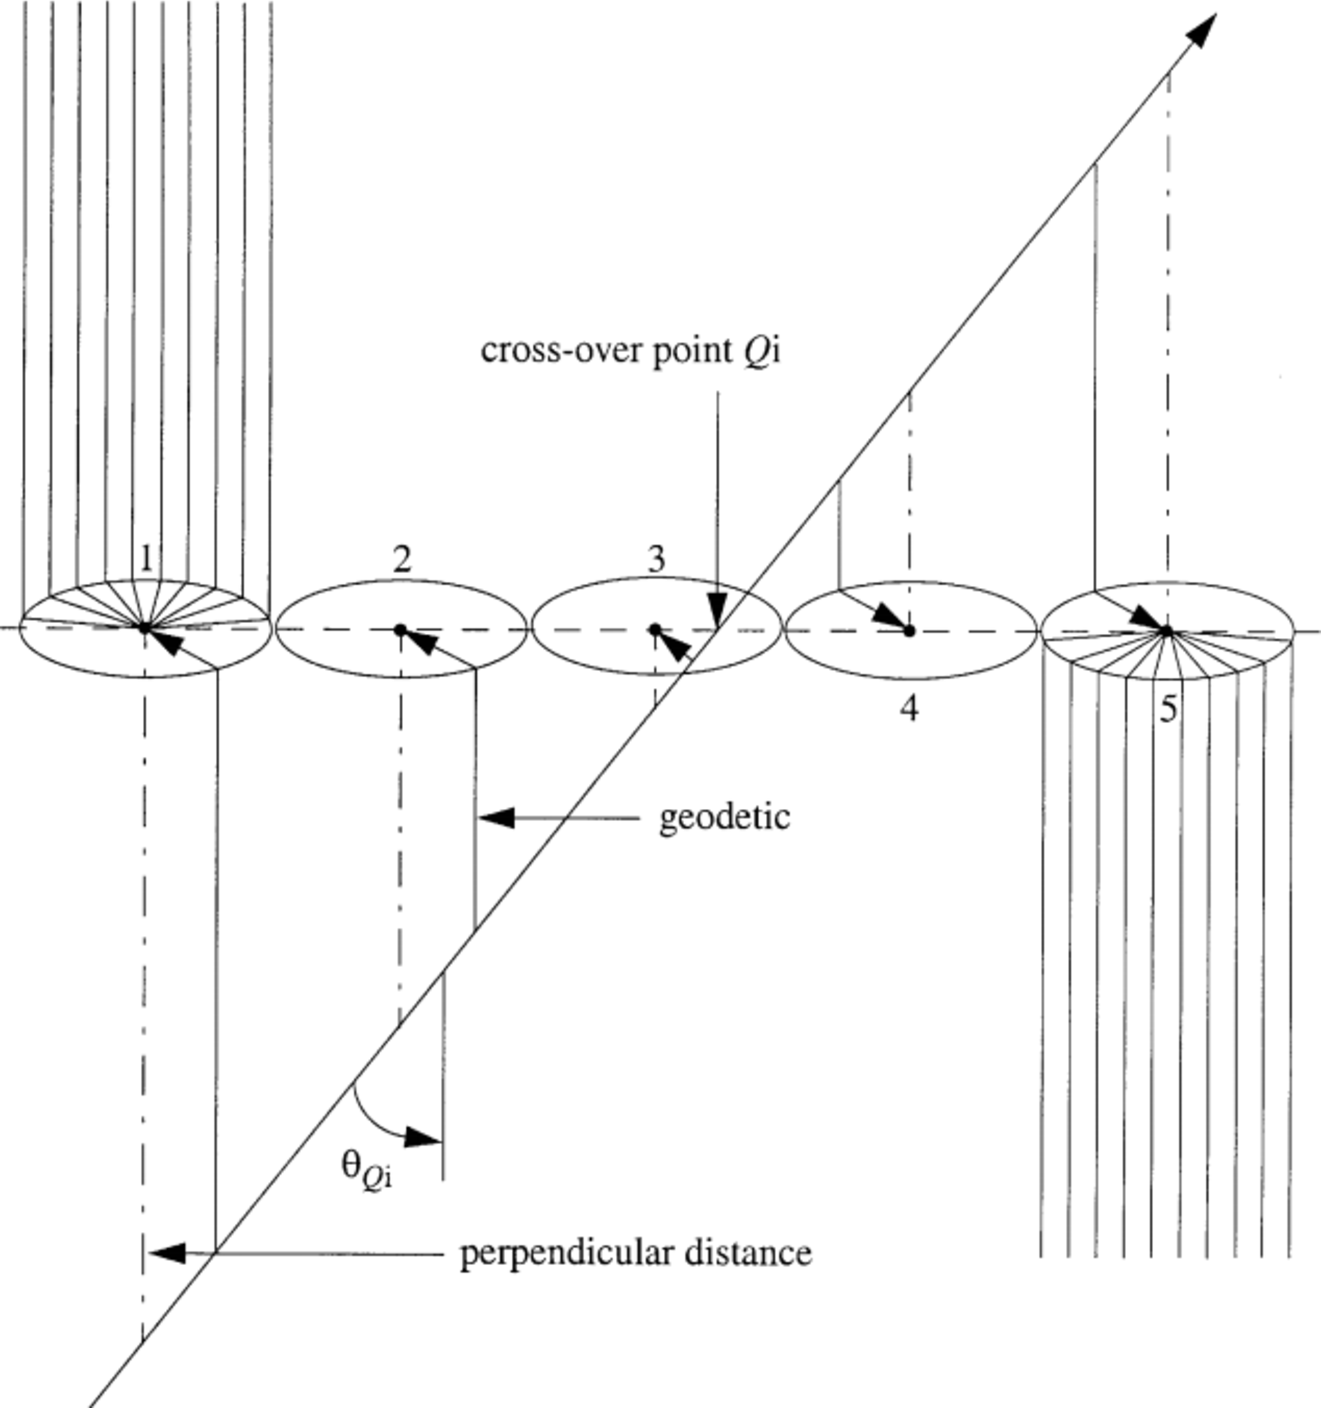
\includegraphics[width=10cm]{VDCpath.pdf}
		\caption{A possible track that causes signals in  wires. The drift electrons will follow the arrow path. The dot/dashed lines correspond to the projected distance used to reconstruct the path of the incident particle. The transition point from parallel to radial field lines is represented by the ellipses. \cite{drift} }
		\label{vdcpath}
	\end{figure}
	\paragraph{}The drift chamber's performance is constantly monitored throughout the experiment. The efficiency of an individual wire is determine by an algorithm that scans a plane for an event that fires a cluster of wires. A wire is determine to be efficient for that event if it fired along with it's two nearest neighbors. This efficiency calculation is used during the online analysis to keep track of the performance of the VDCs and to assistant the maintenance of the HRSs throughout the experiment. 
	\begin{figure}
		\centering
		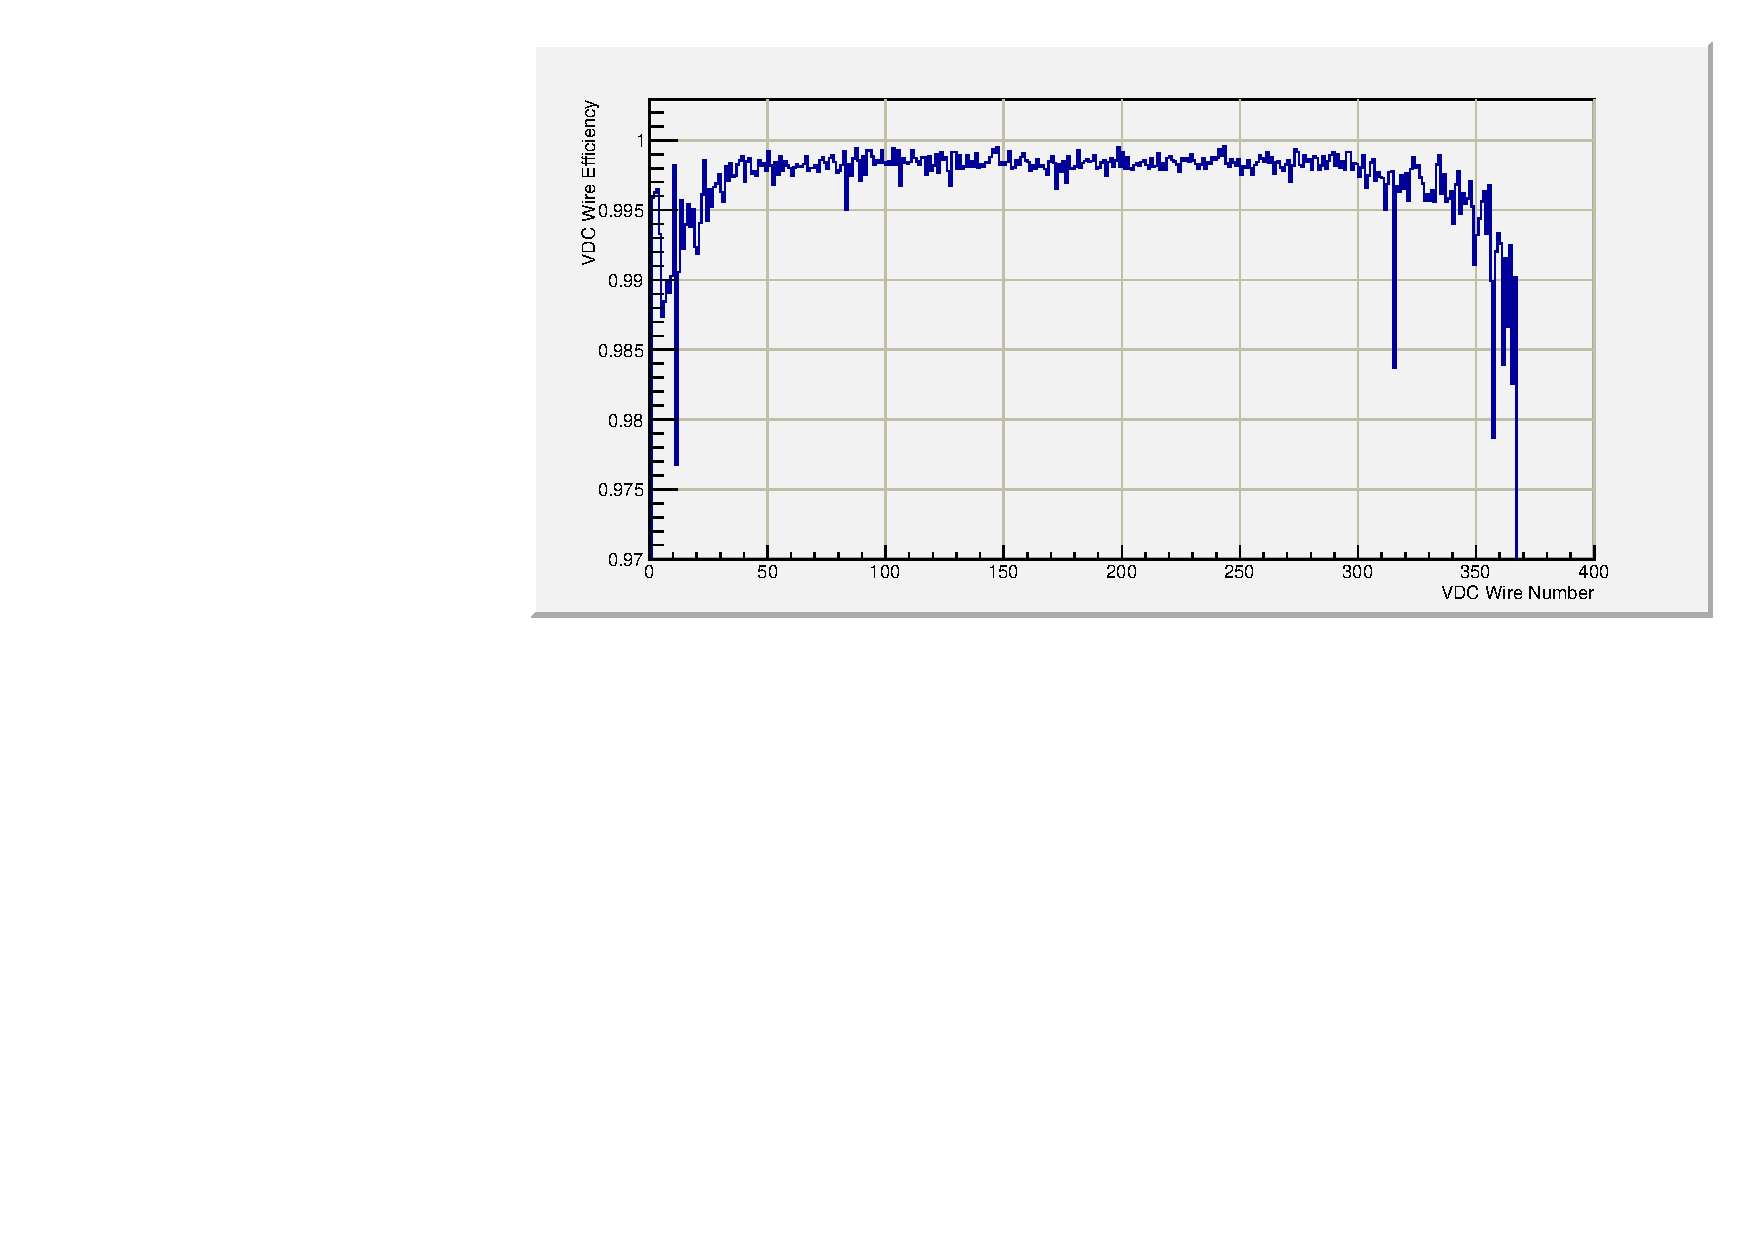
\includegraphics[width=15cm]{VDCeff.pdf}
		\caption{The VDC efficiency for one plane of wires.}
		\label{vdceff}
	\end{figure}
	\paragraph{}The VDC's main task during an electron counting experiment is to determine the track of the scattered electron. The track of the electron is used to ascertain the electron's scattering momentum and scattering angle. Due to the electron's relativistic nature the primary ionization event for each wire region happens simultaneously compared to the resolution of the TDCs. The common stop TDCs used for the VDC signals record the amount of time from drift electron's signal in the sense wires to the stop signal formed by the trigger. This creates a high TDC signal for short drift distances. The raw TDC values recorded by the VDC include time associated with the signal but also the time required to form the trigger and time of flight for electrons between the VDCs and detectors used in the formation of a trigger. The calibration of the VDC removes these extra sources of time in the TDC signal. In order to calibrate the VDC raw signals, a refrense time is determined for every wire on every plane. This references time ($t_0$) is chosen as the TDC value of the sharp decrease on the outside of the peak in region C shown in figure \ref{fig:vdcraw}.
	\begin{figure}[h]
		\centering
		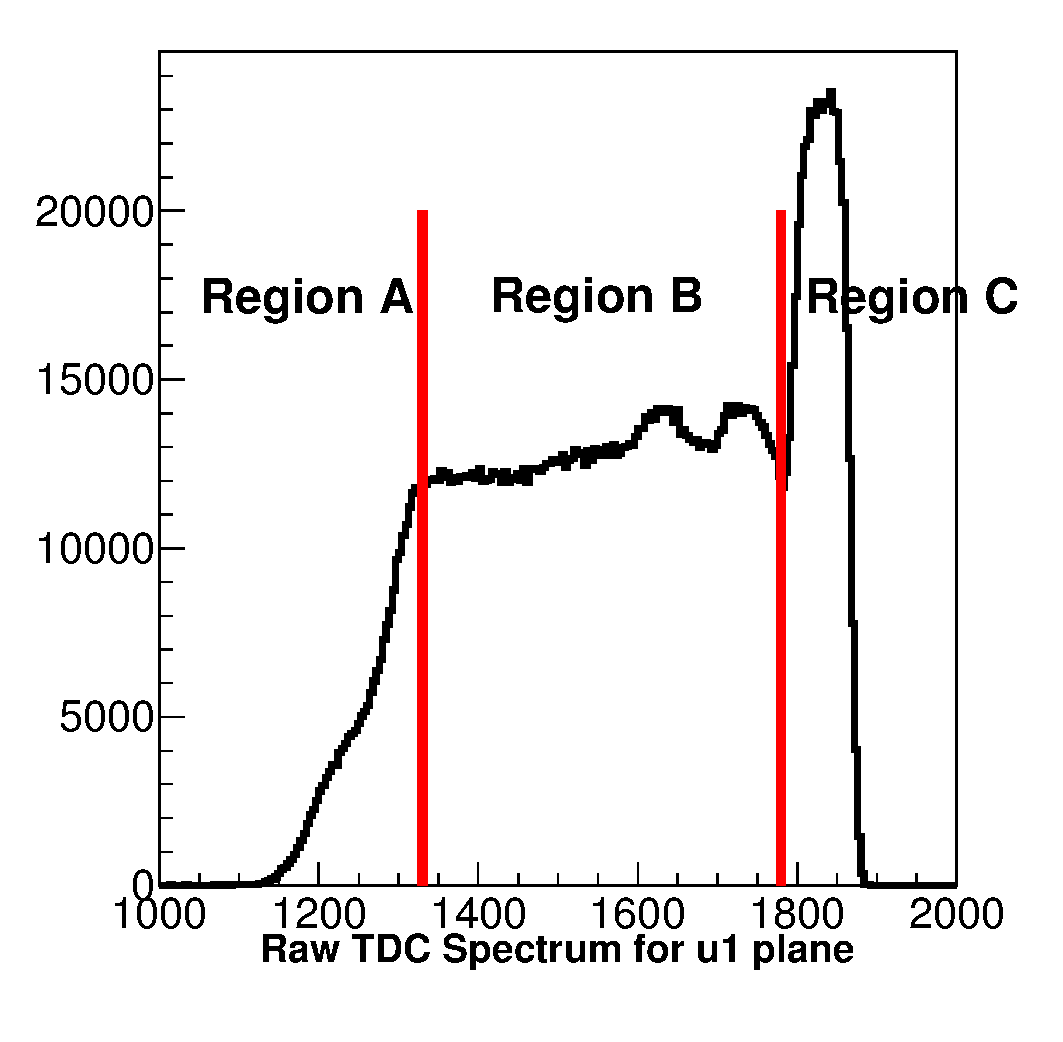
\includegraphics[width=7.5cm]{vdc_raw.pdf}
		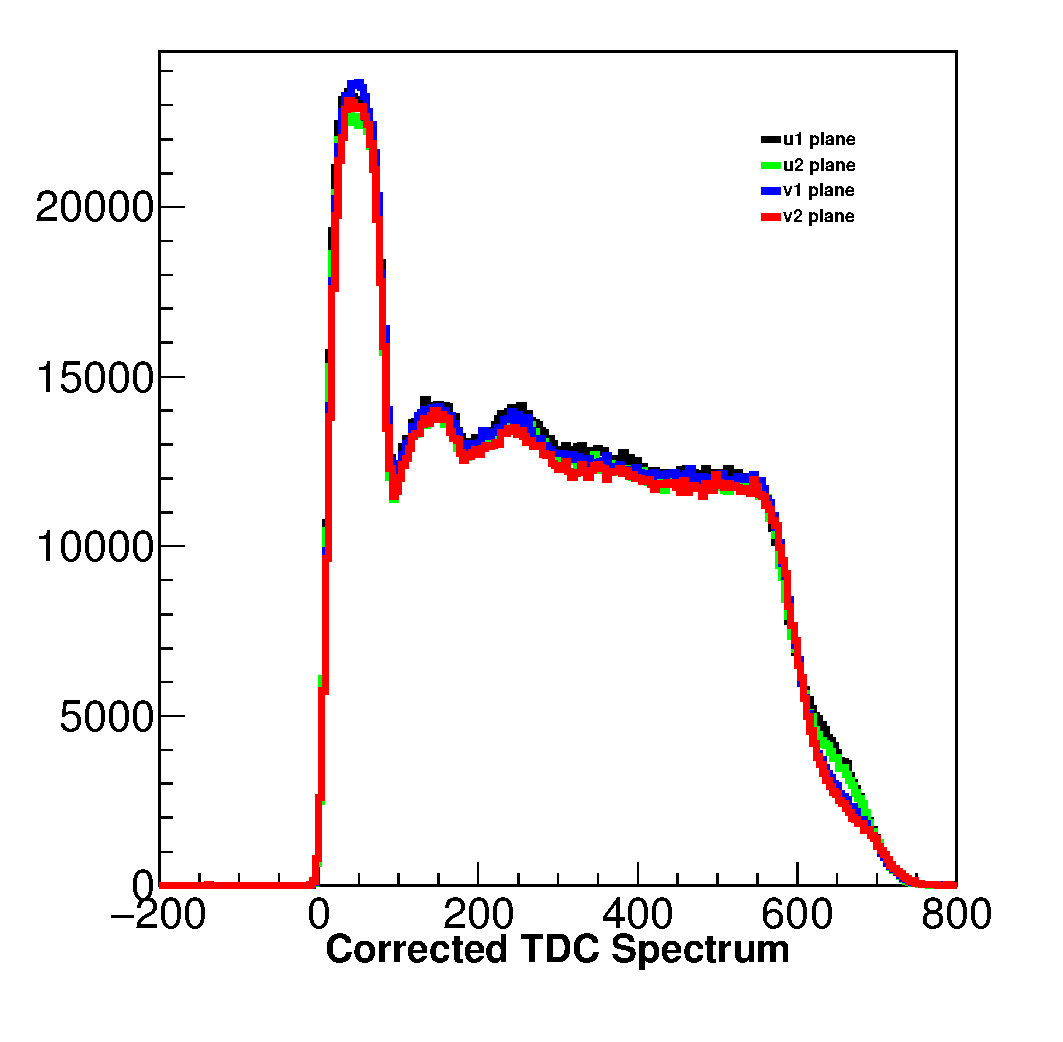
\includegraphics[width=7.5cm]{vdc_cal.pdf}
		\caption{Histograms of VDC signals before(left) and after(right) calibration of t0\cite{primer}.}
		\label{fig:vdcraw}
	\begin{itemize}
		\item Region A: In this region, the point of primary ionization is far from the sense wire. As this distance increases, the chance of detecting the transversing particles by this wire is decreased. 
		\item Region B: The probability of sense wires detecting a primary ionization event in this region are uniform due to the uniform electric field though out the region. 
		\item Region C: The primary ionization position for these events are very near the sense wire and the electric field from this area is going to change to radial shape and the 	probability to detect a particle is going to increase in this area. The sense wire exist in the region, so the ionization event will have a minimum distance. This is shown in the sharp decline on the outside of the peak in region C. 
		\cite{primer}
	\end{itemize}	
	\end{figure}
	The time recorded from the TDCs is used to construct a location of the ionization event for each sense wire across the trajectory of the scattered electron. The analyzing software will use these drift distance from the four VDC planes to find a track for the scattered electron.

	\subsection{Scintillators}\label{sec:scin}
	\paragraph{} A pair of scintillator planes form the primary triggering apparatus for the HRSs. The planes of scintillator S0 and S2 consist of a collection of plastic scintillating paddles with photo multiplier tubes(PMTs) attached to both ends of the paddle. S0 the first scintillator in the stack consist of one scintillating paddle in a vertical direction. S2, the second scintillator was build with 16 overlapping paddles with PMTs attached to both ends. As electrons enter the scintillating plastics energy is absorbed by the material scintillating light. This light is detected by the PMTs on either side of the bar. The passing of the electron can happen at positions at an unequal distances from the PMTs on a scintillator bar. These relative differences cause a distortion in the timing calculation in the TOF known as the time walk effect. The scintillators are used in the calculation of $\beta$, the $v$ to $c$ ratio. Beta is calculated using the time of flight(TOF) between the two scintillator planes and distance traveled between the two points of interaction. 
	\begin{figure}[h]
		\centering
		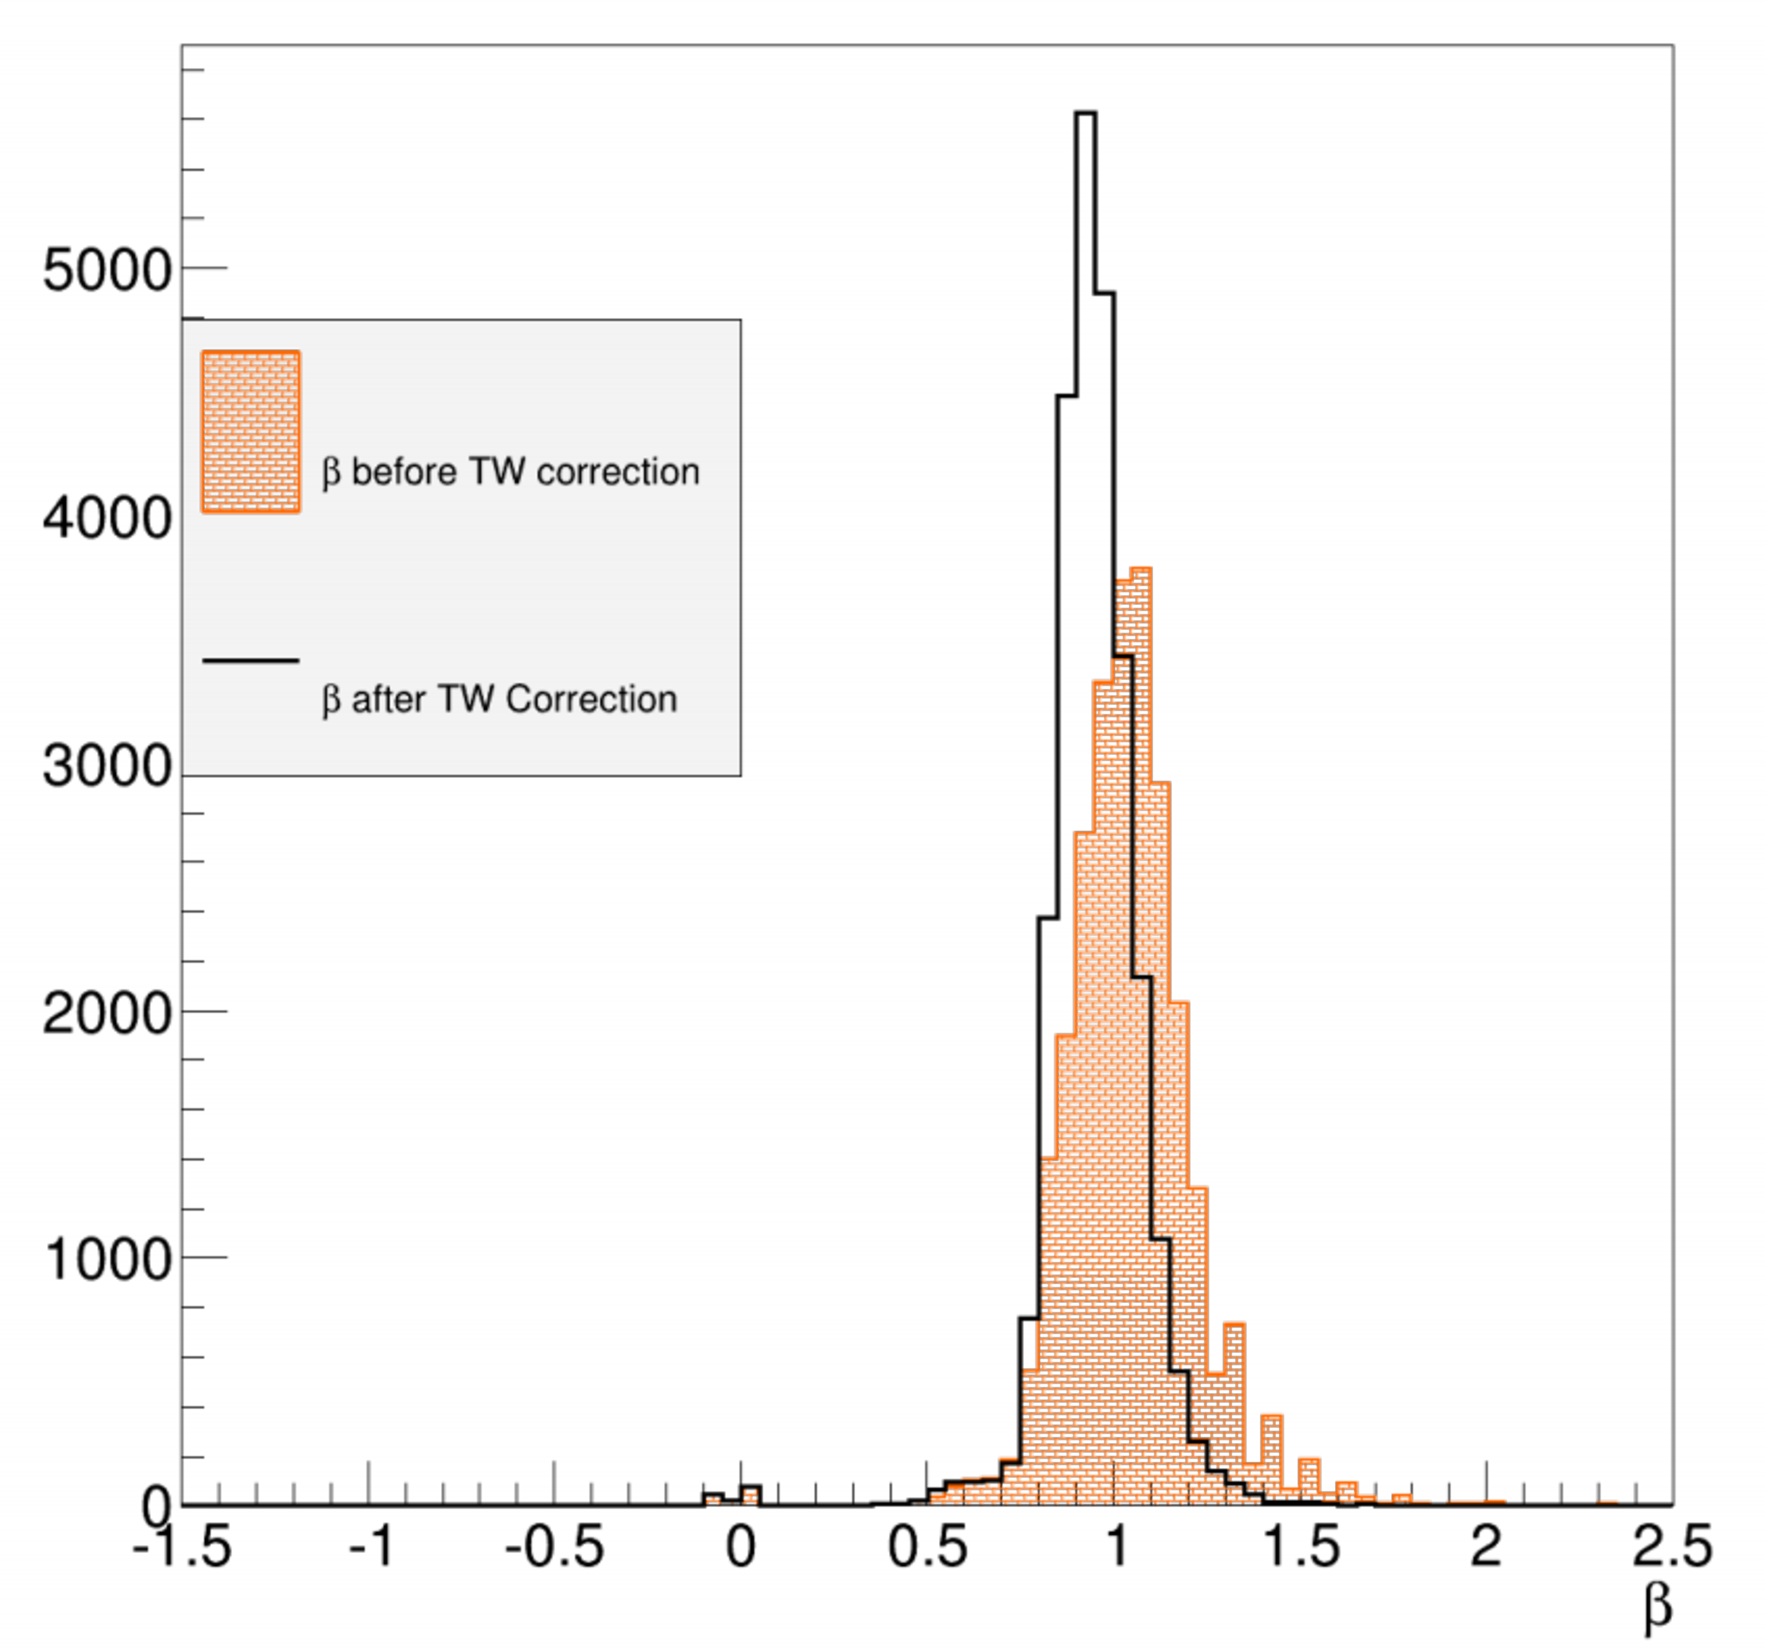
\includegraphics[width=9.5cm]{twcor.pdf}
		\caption{Histogram of $\beta$ before and after time walk correction.}
		\label{fig:twcor}
	\end{figure}
	
	
	\subsection{Cherenkov}\label{sec:Cer}
	\paragraph{}After a particle passes through S0, it will enter the large gas chamber for the gas cherenkov(GC). The GC is filled with $CO_2$ with an index of refraction of 1.00041. This high index of refraction creates a momentum threshold of 0.017 GeV/C for electrons, 4.8 GeV/C for pions, and 32 GeV/c for protons\cite{GasC}. 
	
	If an electron that scatters into the GC is relativistic, 
	\cite{ref:GC}
	
	\subsection{Calorimeter}\label{sec:Cal}


\section{Trigger Setup}\label{sec:Trig}

%\section{DAQ - Data Acquisition System}\label{sec:daq}

\section{Kinematic Settings}\label{sec:kin}









